\begin{refsection}

\chapter{\textsuperscript{230}Th--U}\label{ch:ThU}

The general principles of U-series disequilibrium dating were laid out
in Chapter~\ref{ch:intro2Useries}. Recall that the radioactive decay
of \textsuperscript{238}U to \textsuperscript{206}Pb produces
short-lived \textsuperscript{230}Th (t\textsubscript{1/2}=76~kyr) and
\textsuperscript{234}U (t\textsubscript{1/2}=246~kyr), which may
fractionate by one of several mechanisms:

\begin{enumerate}
\item U and Th have contrasting chemical properties and are easily
  fractionated during chemical processes such as crystallisation. This
  fractionation disrupts any pre-existing state of secular equilibrium
  between \textsuperscript{230}Th and its parent nuclide
  \textsuperscript{234}U.
\item Preferential leaching of weakly sited \textsuperscript{234}U due
  to energetic recoil of the U-nucleus during
  \textsuperscript{238}U-decay enriches \textsuperscript{234}U
  relative to \textsuperscript{238}U in river and sea water.
\item Redox processes and repeated precipitation--dissolution cycles
  may fractionate \textsuperscript{234}U from \textsuperscript{238}U,
  especially in the presence of organic acids in soils. This can
  produce ground waters that are highly enriched in
  \textsuperscript{234}U relative to \textsuperscript{238}U.
\end{enumerate}

Section~\ref{sec:234238} showed that the fractionation between
\textsuperscript{234}U and \textsuperscript{238}U can be used to date
marine carbonates; Section~\ref{sec:230} showed that the fractionation
between \textsuperscript{230}Th and \textsuperscript{234}U can be used
to date young volcanic rocks; and Section~\ref{sec:230238} combined
the two equations together in a single equation. Recall
Equation~\ref{eq:230238}:
\begin{equation*}
  \frac{A(^{230}Th)}{A(^{238}U)} = 1 - e^{-\lambda_{230}t} +
  \frac{\lambda_{230}}{\lambda_{230}-\lambda_{234}} (\gamma_\circ-1)
\left(e^{-\lambda_{234}t}-e^{-\lambda_{230}t}\right)
\end{equation*}

\noindent where $A[\ast]$ is the activity of $\ast$ and $\gamma_\circ$
is the oceanic \textsuperscript{234}U/\textsuperscript{238}U activity
ratio. This equation requires that $\gamma_\circ$ is known and
produces non-unique age solutions when
A(\textsuperscript{230}Th)/A(\textsuperscript{238}U)$>1$. Both of
these limitations can be avoided by recasting the equation into the
following form:
\begin{equation}
  \begin{split}
  & \frac{A[{}^{230}Th] - A[{}^{230}Th]_{\circ}e^{-\lambda_{230}t}}{A[{}^{238}U]} = \\
  & 1 - e^{\lambda_{230}t} -
  \left(\frac{A[{}^{234}U]}{A[{}^{238}U]}-1\right)
  \left(\frac{\lambda_{230}}{\lambda_{234}-\lambda_{230}}\right)
  \left(1-e^{[\lambda_{234}-\lambda_{230}]t}\right)
  \end{split}
  \label{eq:Th-U}
\end{equation}

\noindent where $A[{}^{230}Th]_\circ$ is the `detrital' \textsuperscript{230}Th
component, i.e. the \textsuperscript{230}Th that was already present
in the sample at the time of its formation \citep{kaufman1965,
  ludwig2003b}. This component is unknown but can be estimated by
isochron regression using long-lived \textsuperscript{232}Th as a
normalising factor.\\

\texttt{IsoplotR} uses Equation~\ref{eq:Th-U} as the basis of all its
U-series dating applications.

\section{Data formats}\label{sec:ThUformats}

\texttt{IsoplotR} accepts U-series data in four different formats:

\begin{enumerate}
\item $\frac{38}{32}$, $s\!\left[\frac{38}{32}\right]$,
  $\frac{34}{32}$, $s\!\left[\frac{34}{32}\right]$,
  $\frac{30}{32}$, $s\!\left[\frac{30}{32}\right]$,
  $r\!\left[\frac{38}{32},\frac{34}{32}\right]$,
  $r\!\left[\frac{38}{32},\frac{30}{32}\right]$,
  $r\!\left[\frac{34}{32},\frac{30}{32}\right]$
\item $\frac{32}{38}$, $s\!\left[\frac{32}{38}\right]$,
  $\frac{34}{38}$, $s\!\left[\frac{34}{38}\right]$,
  $\frac{30}{38}$, $s\!\left[\frac{30}{38}\right]$,
  $r\!\left[\frac{32}{38},\frac{34}{38}\right]$,
  $r\!\left[\frac{32}{38},\frac{30}{38}\right]$,
  $r\!\left[\frac{34}{38},\frac{30}{38}\right]$
\item $\frac{38}{32}$, $s\!\left[\frac{38}{32}\right]$,
  $\frac{30}{32}$, $s\!\left[\frac{30}{32}\right]$,
  $r\!\left[\frac{38}{32},\frac{30}{32}\right]$
\item $\frac{32}{38}$, $s\!\left[\frac{32}{38}\right]$,
  $\frac{30}{38}$, $s\!\left[\frac{30}{38}\right]$,
  $r\!\left[\frac{32}{38},\frac{30}{38}\right]$
\end{enumerate}

\noindent where `30', `32', `34' and `38' stand for
\textsuperscript{230}Th, \textsuperscript{232}Th,
\textsuperscript{234}U and \textsuperscript{238}U, respectively.  It
is important to emphasise that, unlike all of \texttt{IsoplotR}'s
other data formats, the numbers in these data tables are no atomic
ratios but activity ratios. The relationship between activity ratios
and atomic ratios is given by:
\begin{equation}
  \frac{A(x)}{A(y)} \equiv 
  \frac{\mbox{activity}(x)}{\mbox{activity}(y)} =
  \frac{\mbox{atoms}(x)}{\mbox{atoms}(y)}
  \frac{\lambda_{x}}{\lambda_{y}}
\end{equation}

Formats~1 and 2 are applicable to carbonate lithologies in which both
the \textsuperscript{230}Th/\textsuperscript{234}U and
\textsuperscript{234}U/\textsuperscript{238}U equilibrium have been
disturbed. Formats~3 and 4 are applicable to igneous rocks, in which
only the \textsuperscript{230}Th/\textsuperscript{234}U activity ratio
has been distrubed, but \textsuperscript{234}U and
\textsuperscript{238}U are in secular equilibrium (see
Section~\ref{sec:230}).

The error correlations of formats~1 and 3 tend to be stronger than
those of formats~2 and 4. This is because formats~1 and 3 normalise
the elements of the \textsuperscript{238}U decay series to the highly
variable amount of detrital \textsuperscript{232}Th. In contrast,
formats~2 and 4 feature only one ratio containing
\textsuperscript{232}Th, thus reducing a source of shared variability.

\section{Isochrons}

For igneous samples, in which $A[{}^{234}U]/A[{}^{238}U] = 1$, the
second term on the right-hand side of Equation~\ref{eq:Th-U} vanishes
and we can write:
\begin{equation}
  \left(\frac{A[{}^{230}Th]}{A[{}^{232}Th]}\right)_i = 
  \left(\frac{A[{}^{230}Th]}{A[{}^{232}Th]}\right)_{\!\circ}
  e^{-\lambda_{230}t} +
  \left(\frac{A[{}^{238}U]}{A[{}^{232}Th]}\right)_i
  \left(1-e^{-\lambda_{230}t}\right)
  \label{eq:rosholt}
\end{equation}

\noindent for $1 \leq i \leq n$, which can be solved for $t$ and
$\left(A[{}^{230}Th]/A[{}^{232}Th]\right)_{\!\circ}$ using the least
squares method of \citet{york2004}. Equation~\ref{eq:rosholt} (which
was previously derived as Equation~\ref{eq:230232}) forms a
`Rosholt'-type isochron, which is akin to a conventional isochron in
Rb--Sr or Ar--Ar geochronology \citep{rosholt1976}. Using
$A[{}^{238}U]$ as the normalising factor instead yields an
`Osmond'-type isochron, which is akin to an inverse isochron in Ar--Ar
or Pb--Pb geochronology \citep{osmond1970, ludwig2003b}:
\begin{equation}
  \left(\frac{A[{}^{230}Th]}{A[{}^{238}U]}\right)_i =
  \left(1-e^{\lambda_{230}t}\right) +
  \left(\frac{A[{}^{232}Th]}{A[{}^{238}U]}\right)_i
  \left(\frac{A[{}^{230}Th]}{A[{}^{232}Th]}\right)_\circ
  e^{-\lambda_{230}t}
  \label{eq:osmond}
\end{equation}

Note that for the Rosholt isochron, the age is a function of the
slope, whereas for the Osmond isochron, it is a function of the
y-intercept.\\

For carbonate samples, in which \textsuperscript{234}U and
\textsuperscript{238}U generally are not in secular equilibrium, three
activity ratios are needed to determine the detrital
\textsuperscript{230}Th (and initial \textsuperscript{234}U)
component. This in turn requires three dimensional isochron regression
of the \textsuperscript{230}Th/\textsuperscript{238}U-,
\textsuperscript{232}Th/\textsuperscript{238}U- and
\textsuperscript{234}U/\textsuperscript{238}U-activity
ratios. \texttt{IsoplotR} performs this calculation using the maximum
likelihood algorithm of \citet{ludwig1994}. This solves the following
system of equations\footnote{The same calculations can also be
performed in `Rosholt space', with \textsuperscript{232}Th as a common
denominator, but an in-depth discussion of this is omitted for the
sake of brevity.}:
\begin{equation}
  \begin{cases}
    \left[\frac{{}^{234}\mbox{U}}{{}^{238}\mbox{U}}\right]_i =
    a + b \left[\frac{{}^{232}\mbox{Th}}{{}^{238}\mbox{U}}\right]_i +
    \delta_i \\
    \left[\frac{{}^{230}\mbox{Th}}{{}^{238}\mbox{U}}\right]_i =
    \alpha + \beta \left[\frac{{}^{232}\mbox{Th}}{{}^{238}\mbox{U}}\right]_i +
    \epsilon_i
  \end{cases}
  \label{eq:titterington}
\end{equation}

\noindent where $\delta_i$ and $\epsilon_i$ are the bivariate normal
residuals. Equation~\ref{eq:titterington} can be solved by maximising
the following log-likelihood function for $x_i$, $a$, $b$, $\alpha$
and $\beta$:
\begin{equation}
  \mathcal{LL} = \mbox{const.} - 
  \frac{1}{2} \sum\limits_{i=1}^{n}
  \left[
    \begin{array}{@{}c@{}}
      \left[\frac{32}{38}\right]_{\!i} - x_{i} \\
      \left[\frac{34}{38}\right]_{\!i} - a - b x_{i} \\
      \left[\frac{30}{38}\right]_{\!i} - \alpha - \beta x_{i}
    \end{array}
    \right]^T
  \left[
    \begin{array}{@{}c@{~}c@{~}c@{}}
      s\!\left[\frac{32}{38}\right]_{\!i}^2 &
      s\!\left[\frac{32}{38},\frac{34}{38}\right]_{\!i} &
      s\!\left[\frac{32}{38},\frac{30}{38}\right]_{\!i} \\
      s\!\left[\frac{34}{38},\frac{32}{38}\right]_{\!i} &
      s\!\left[\frac{34}{38}\right]_{\!i}^2 &
      s\!\left[\frac{34}{38},\frac{30}{38}\right]_{\!i} \\
      s\!\left[\frac{30}{38},\frac{32}{38}\right]_{\!i} &
      s\!\left[\frac{30}{38},\frac{34}{38}\right]_{\!i} &
      s\!\left[\frac{30}{38}\right]_{\!i}^2
    \end{array}
    \right]^{-1}
  \left[
    \begin{array}{@{}c@{}}
      \left[\frac{32}{38}\right]_{\!i} - x_{\!i} \\
      \left[\frac{34}{38}\right]_{\!i} - a - b x_{i} \\
      \left[\frac{30}{38}\right]_{\!i} - A - B x_{i}
    \end{array}
    \right]
\end{equation}

\noindent which uses the shorthand notation introduced at the
beginning of Section~\ref{sec:ThUformats}. The isochron age can be
obtained by substituting the estimate of $a$ for
$\left[\frac{{}^{234}\mbox{U}}{{}^{238}\mbox{U}}\right]_i$ and
$\alpha$ for
$\left[\frac{{}^{230}\mbox{Th}}{{}^{238}\mbox{U}}\right]_i$ in
Equation~\ref{eq:Th-U}, and setting $A[{}^{230}Th]_{\circ}=0$.
Additionally, the fit parameters ($a$, $b$, $\alpha$ and $\beta$) can
also be used to estimate the following quantities:

\begin{enumerate}
\item{(\textsuperscript{234}U/\textsuperscript{238}U)\textsubscript{0}} $=a$:
  the authigenic \textsuperscript{234}U/\textsuperscript{238}U
  activity ratio;
\item{(\textsuperscript{230}Th/\textsuperscript{232}Th)\textsubscript{0}}
  $=\beta$: the authigenic
  \textsuperscript{230}Th/\textsuperscript{232}Th activity ratio;
\item{(\textsuperscript{230}Th/\textsuperscript{238}U)\textsubscript{0}}
  $=\alpha$: the detrital
  \textsuperscript{230}Th/\textsuperscript{238}U activity ratio;
\item{(\textsuperscript{234}U/\textsuperscript{238}U)\textsubscript{i}}
  = $1 + (a-1)e^{\lambda_{234}t}$: the initial
  \textsuperscript{234}U/\textsuperscript{238}U activity ratio.
\end{enumerate}

The results of the three-dimensional isochron regression can be
visualised in four possible ways:

\noindent\begin{minipage}[t][][b]{.65\linewidth}
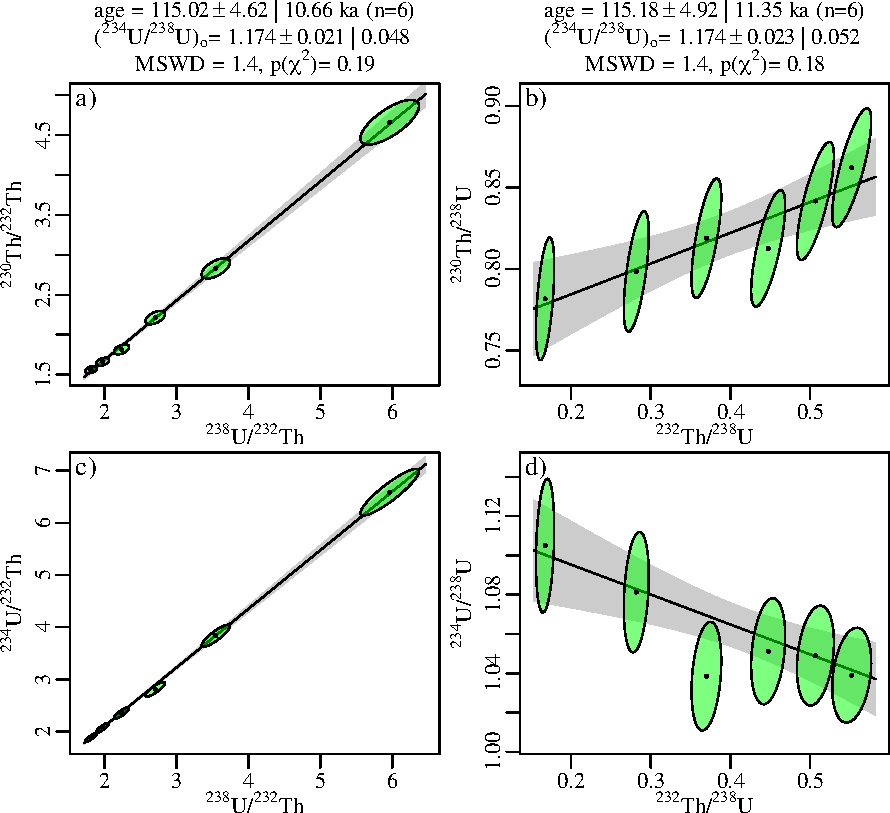
\includegraphics[width=\textwidth]{../figures/ThUisochron.pdf}
\end{minipage}
\begin{minipage}[t][][t]{.35\linewidth}
  \captionof{figure}{The same \textsuperscript{230}Th--U data shown on
    a) Rosholt type-I, b) Osmond type-I, c) Rosholt type-II and d)
    Osmond type-II isochron diagrams. Note the slight difference in
    the isochron age. This is due to the skewness of the uncertainty
    distribution, which does not allow negative values.  This effect
    applies to all isochrons and is most prominent when the analytical
    uncertainties are relatively large compared to the activity ratios
    themselves. Solving this issue requires a reformulation of the
    isochron equation in terms of log-ratios, which has not yet been
    attempted.}
  \label{fig:ThUisochron}
\end{minipage}

\section{Th--U evolution diagrams}\label{sec:ThUevolution}

In addition to (Rosholt and Osmond) isochrons and the usual weighted
mean, radial, CAD and KDE plots, U-series data can also be visualised
on Th-U evolution diagrams.  For carbonate data, these consist of a
scatter plot that sets out the
\textsuperscript{234}U/\textsuperscript{238}U-activity ratios against
the \textsuperscript{230}Th/\textsuperscript{238}U-activity ratios as
error ellipses, and displays the authigenic
\textsuperscript{234}U/\textsuperscript{238}U-activity ratios and ages
as a set of intersecting lines.\\

The Th-U evolution diagram has a similar purpose and appearance as the
U-Pb concordia diagram (Section~\ref{sec:concordia}), which also
displays compositions and dates simultaneously. An alternative way of
doing so for carbonate samples is by plotting the initial
\textsuperscript{234}U/\textsuperscript{238}U-ratios against the
\textsuperscript{230}Th--\textsuperscript{234}U--\textsuperscript{238}U-ages.
In both types of evolution diagrams, \texttt{IsoplotR} provides the
option to project the raw measurements along the best fitting isochron
line and thereby remove the detrital
\textsuperscript{230}Th-component. This procedure allows a visual
assessment of the degree of homogeneity within a dataset, as
quantified by the MSWD.\medskip

\noindent
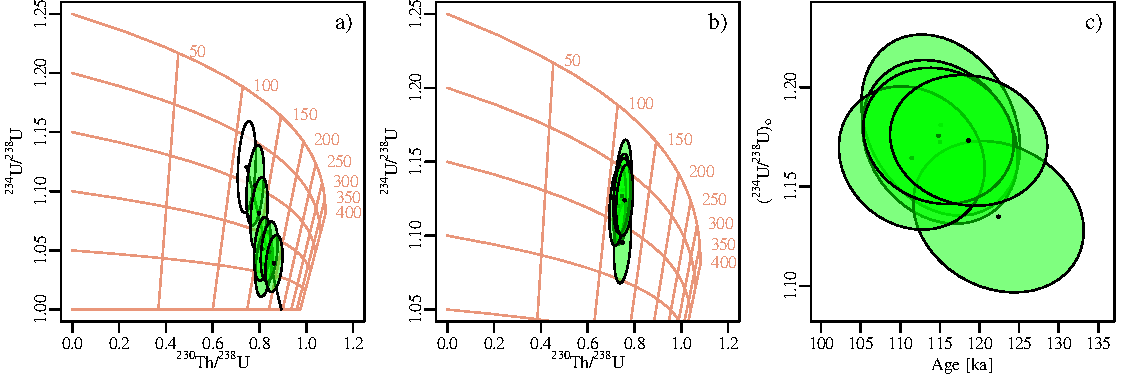
\includegraphics[width=\linewidth]{../figures/evolution12.pdf}
\captionof{figure}{The data of Figure~\ref{fig:ThUisochron}
  visualised on a \textsuperscript{230}Th--U evolution diagram a)
  showing the raw data with an isochron fit and the inferred
  authigenic end member composition shown as a white ellipse; and b)
  showing the data projected along the isochron.  c) shows the
  projected data in initial
  \textsuperscript{234}U/\textsuperscript{238}U-activity
  vs. \textsuperscript{230}Th--U age space.\medskip}
\label{fig:evolution12}

Neither the U-series evolution diagram nor the
\textsuperscript{234}U/\textsuperscript{238}U vs. age plot is
applicable to igneous datasets, in which \textsuperscript{234}U and
\textsuperscript{238}U are in secular equilibrium.  For such datasets,
\texttt{IsoplotR} produces an Rosholt type-I style regression plot
that is decorated with a fanning set of isochron lines.\medskip

\noindent\begin{minipage}[t][][b]{.7\linewidth}
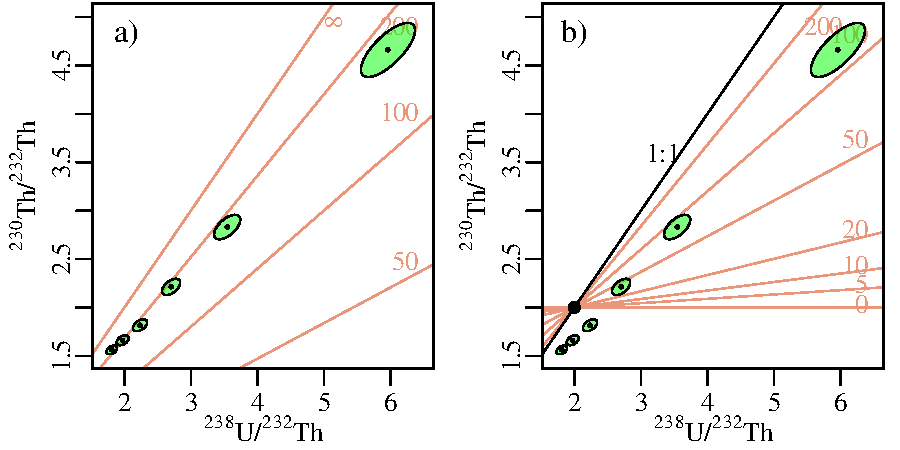
\includegraphics[width=\textwidth]{../figures/evolution34.pdf}
\end{minipage}
\begin{minipage}[t][][t]{.29\linewidth}
  \captionof{figure}{ An evolution diagram of data formats~3 and 4
    plots the data in Rosholt type-I space with isochrons shown in
    salmon red a) without detrital \textsuperscript{230}Th correction;
    and b) using a whole rock U/Th activity ratio of 2 to estimate the
    \textsuperscript{230}Th/\textsuperscript{238}U isochron ratios.}
  \label{fig:evolution34}
\end{minipage}

\printbibliography[heading=subbibliography]

\end{refsection}
